\section{Middleware \textit{uOS}}
\label{uos}

	O Middleware \textit{uOS}~\cite{fabriciobuzzeto} é um projeto do grupo de pesquisa \textit{UnBiquitous}\footnote{Este trabalho é parte integrante do projeto \textit{UnBiquitous}} da Universidade de Brasília cujo foco está na adaptabilidade de serviços em um ambiente de computação ubíqua, de modo que os serviços dos dispositivos presentes no ambiente possam ser oferecidos e compartilhados.

	 O \textit{uOS} é uma implementação de um middleware para auxílio de aplicações para ambiente de computação ubíquoa, cuja proposta é compatível com os conceitos apresentados pela \textit{DSOA} (\textit{Device Service Oriented Architecture})~\cite{fabriciobuzzeto}. 
	 % Seguindo a arquitetura \textit{SOA} (\textit{Service Oriented Architecture}) a \textit{DSOA} também possui os papéis de consumidor, provedor e registro; com a diferença de que na \textit{DSOA} quem assume esses papéis são os dispositivos e não os \textit{Web Services}.

	 \begin{figure}[htb]
		\begin{center}
			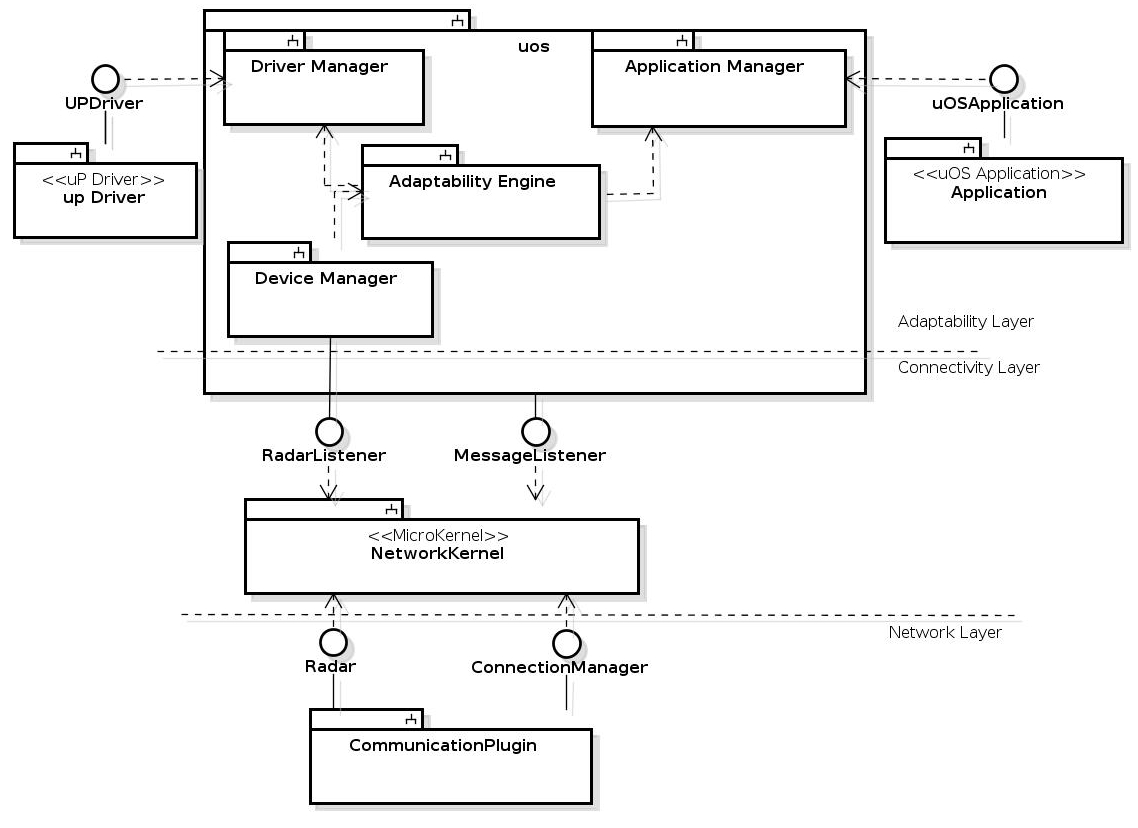
\includegraphics[scale=0.45]{figuras/4.ProblemaEProposta/uoscamadas.jpg}
		\end{center}
		\caption{Camadas do middleware \textit{uOS}.}
		\label{fig:arq-uos}
	\end{figure}

	A Figura~\ref{fig:arq-uos} mostra as três camadas do middleware \textit{uOS}:

	\begin{enumerate}
		\item Camada de Rede: responsável por gerenciar as interfaces de rede do dispositivo;
		\item Camada de Conectividade: responsável por gerenciar conexões entre dispositivo que se comunicam por diferentes tecnologias, como Bluetooth e Ethernet;
		\item Camada de Adaptabilidade: responsável por gerenciar os serviços disponíveis e o acesso aos mesmos.
	\end{enumerate}

	A camada de Rede contém os módulos: RADAR e \textit{Connection Manager}. O RADAR descobre os dispositivos do ambiente por meio de varreduras e o \textit{Connection Manager} gerencia conexões entre dispositivos com a mesma tecnologia de comunicação. Na camada de Conectividade, a comunicação entre dispositivos com diferentes tecnologias é obtida com a utilização de um Proxy. Por fim, a camada de Adaptabilidade contém um módulo chamado \textit{Adaptability Engine}, que faz a intermediação entre as aplicações e os \textit{drivers} com o objetivo de selecionar o serviço mais apropriado para determinada aplicação. A camada de Adaptabilidade também contém o módulo \textit{Application Deployer}, que permite a inclusão e exclusão de aplicações por meio das operações de \textit{Deploy} e \textit{Undeploy}.

	A integração do Sistema TRUE com o middleware \textit{uOS} foi realizada na Camada de Adaptabilidade através da implementação de um \textit{driver} de ``usuário''. Este \textit{driver} se comunica com o Sistema TRUE disponibilizando as informações colhidas pelo sistema as aplicações no ambiente por meio de serviços. Esta integração será apresentada em detalhes na Seção~\ref{sec:modulo-integracao}.

	% O \textit{UbiquitOS} é uma implementação de um middleware para auxílio de aplicações para ambiente de computação ubíquoa, cuja proposta é compatível com os conceitos apresentados pela \textit{DSOA} (\textit{Device Service Oriented Architecture})~\cite{fabriciobuzzeto}. Este é visto como um componente de auxílio para desenvolvimento de drivers de recurso, aplicações e \textit{plugins} de rede a serem utilizados em ambientes ubíquos~\cite{fabriciobuzzeto}.

	% Um recurso é um grupo de funcionalidades de um dispositivo logicamente relacionadas acessíveis através de interfaces pré-definidas. Tais funcionalidades, por sua vez, são representadas no ambiente através de serviços relacionados~\cite{fabriciobuzzeto}.

	% Uma aplicação é a implementação de um conjunto de comportamentos e regras relacionadas ao ambiente inteligente, cujo o objetivo é a tomada de ação ou a interação junto ao usuário. As aplicações ficam no dispositivos do ambiente e se utilizam dos recursos e serviços do mesmo durante a execução~\cite{fabriciobuzzeto}.

